% Drawing 74/02-8 -- folder 74, batch 02, archive page 29 (PDF page 30).
% Transcription: un segment divisé en deux.
% Kind: segment divided in two. Method 3 (encoded, rendered from the data). Status: ok.
% Notes: A segment with three ticks, i.e. two sub-segments. Encoded as segment-config/1.
% Coordinates: 1 unit = 1 mm = 1/100 of the crop width (bbox in page fractions: [0.3, 0.07, 0.6, 0.13]).
% Redrawn by Claude (claude-opus-5-5), issue #73, 2026-11-07; not checked by a human; not compiled (no TeX in the session).
% Rights: reproduces part of the work -- behind RENDER_TRANSCRIPTS, never published by itself.
\documentclass[tikz,border=3pt]{standalone}
\usepackage{amsmath,amssymb}
\usetikzlibrary{patterns,arrows.meta}
\tikzset{pencil/.style={black!45}, struck/.style={black!35}, mark/.style={circle,draw,inner sep=1.3pt}, pt/.style={circle,fill,inner sep=0.9pt}, opt/.style={circle,draw,fill=white,inner sep=1.1pt}}
\begin{document}
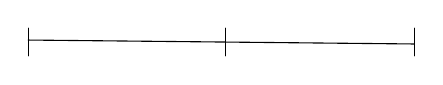
\begin{tikzpicture}[x=1mm,y=1mm,line cap=round,line join=round,font=\scriptsize]
\draw (17,-10) -- (66,-10.5);
\draw (17,-8.5) -- (17,-12);
\draw (42,-8.5) -- (42,-12);
\draw (66,-8.5) -- (66,-12);
\end{tikzpicture}
\end{document}
